\chapter{System topology}
%利用热力学原理进行定性分析。提炼出创新点。
\section{System topology design}
%\subsection{Basic systems}
%\label{sec:bs}

The objective of this research is to research the equipment of solar thermal power generation system, to propose, develop and optimize a solar thermal cascade system depending on the advantages and disadvantages of the solar thermal power generation systems. 
The research is based on the national cooperation project "Collaborative research on key technologies to produce electricity by cascade utilization solar thermal energy" as the background. 
There are three kinds of mature technologies been applied commercially -- parabolic trough, parabolic dish and solar tower. 
Considering the future deployment of solar cascade demo system, two solar thermal technologies, parabolic trough and parabolic dish, are chosen as the basic systems for the design of cascade solar thermal power system. For the cascade utilization of the high temperature of the parabolic receiver, air (or nitrogen) is used as the HTF to transfer the heat collected.
Figure~\ref{fig:PTPD} shows the schematic diagrams of a parabolic trough system and a parabolic dish system.

\begin{figure}[!ht]
\centering
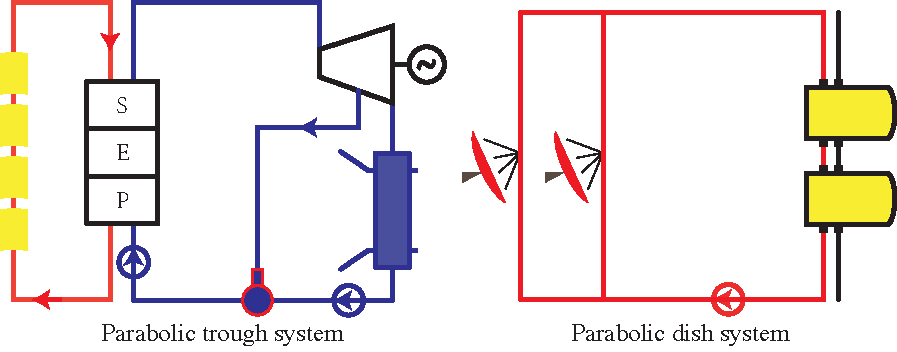
\includegraphics[width=0.8\textwidth]{fig/PTPD.pdf}
\caption{Schematic diagrams of a parabolic trough system and a parabolic dish system}\label{fig:PTPD}
\end{figure}

With different considerations (such as water Rankine cycle or ORC, combination of different systems, connection types of collectors, etc) of the cascade system topology, multiple combination topologies may be used for cascade systems. To get the most suitable system topology, these considerations will be analyzed in the following sections. 

\subsection{Rankine cycle fluid}
\label{sec:RankineCycleFluid}

\begin{figure}[!ht]
\centering 
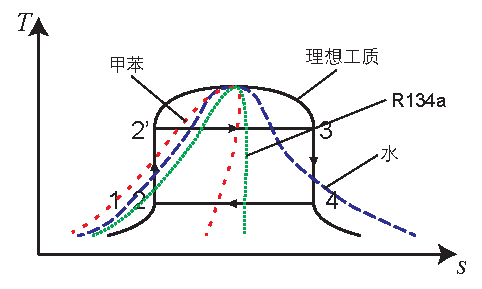
\includegraphics[width=0.7\textwidth]{fig/idealTs}
\caption{Collector and Rankine cycle efficiency variation with operating temperature}\label{fig:idealTs}
\end{figure}

An ideal working fluid would have the temperature entropy diagram given in Figure~\ref{fig:idealTs}. The following characteristics listed by Abbin and Leuenberger~\cite{Abbin1977} describe this fluid:
\begin{itemize}
  \item The heat capacity of the liquid phase should be small. This makes the curve 22' in Figure~\ref{fig:idealTs} almost vertical.
  \item The critical point should be above the highest operating temperature to allow all heat to be added at that temperature.
  \item The vapor pressure at the highest operating temperature should be moderate for safety reasons and to reduce the cost of the equipment.
  \item The vapor pressure at the condensing temperature should be above atmospheric pressure to prevent air leakage into the system.
  \item The specific volume of the vapor at state 4 should be small to avoid large-diameter turbine wheels, casings, and heat exchangers.
  \item The saturated vapor curve 3-4 in Figure~\ref{fig:idealTs} should be vertical to avoid expansion into the wet vapor region (negative $ds/dT$) or expansion into the superheat region (positive $ds/dT$).
  \item For low-power turbine applications, the fluid should have a high molecular weight to minimize the rotational speed and/or the number of turbine stages and to allow for reasonable mass flow rates and turbine nozzle areas.
  \item The fluid should be liquid at atmospheric pressure and temperature for ease of handling and containment.
  \item The freezing point should be lower than the lowest ambient operating temperature.
  \item The fluid should have good heat-transfer properties, be inexpensive, thermally stable at the highest operating temperature, nonflammable, noncorrosive, nontoxic, and so on.
\end{itemize}

Water is the most commonly used fluid for Rankine cycle, it is mare mature to design Rankine cycle components for steam systems than any other liquid. It is inexpensive to use (although boiler-grade water must be highly distilled and thus costs more than tap water), sealing of the high-pressure portions of a Rankine cycle using steam is not critical. Non-flammability and ready availability of steam are additional advantages. Because it has a critical temperature and pressure of 374$\mathrm{^\circ C}$ / 22.1$\mathrm{MPa}$, it can be used for systems operating at fairly high temperatures with most of the heat addition (at constant temperature) and at moderate pressure. Figure~\ref{fig:TypicalSteamRankineSolarSystem} shows the schematic diagram of a typical steam Rankine cycle solar system.

\noindent \begin{figure}[htbp]
\centering
	\begin{subfigure}[b]{0.4\columnwidth}
	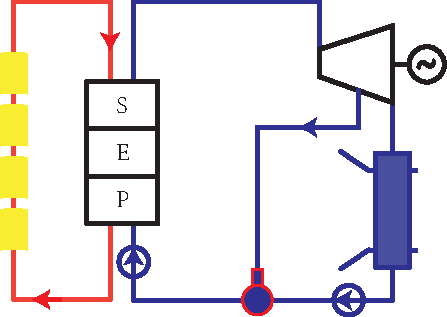
\includegraphics[width = \columnwidth]{fig/TypicalSteamRankineSolarSystem}
	\caption{}\label{fig:TypicalSteamRankineSolarSystem}
	\end{subfigure}
	~
\begin{subfigure}[b]{0.4\columnwidth}
	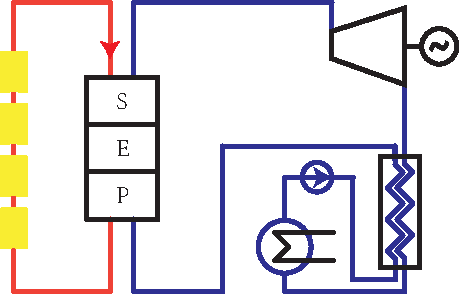
\includegraphics[width = \columnwidth]{fig/TypicalOrganicRankineSolarSystem}
	\caption{}\label{fig:TypicalOrganicRankineSolarSystem}
	\end{subfigure}
	\caption{Schematic diagrams of two types of Rankine cycle solar system}
	\label{fig:TwoTypesOfRankineCycle}
\end{figure}

%\begin{figure}[!ht]
%\centering 
%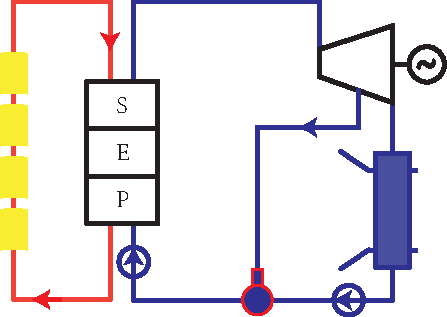
\includegraphics[width=0.7\textwidth]{fig/TypicalSteamRankineSolarSystem}
%\caption{Schematic diagram of a typical steam Rankine cycle solar system}\label{fig:TypicalSteamRankineSolarSystem}
%\end{figure}

There are some disadvantages for steam as the Rankine cycle fluid. The low temperature characteristics of steam are not ideal because the steam has a low vapor pressure (see Table~\ref{tab:waterT_P}) and a very low density at ambient temperature. Therefore, sealing air from low pressure components is a major design problem.
\begin{table}[htbp]
	\caption{Saturated steam pressure at the corresponding temperature}
	\begin{center}
	\begin{tabular}{cccccccccc}
		\toprule	
		    $T$(K)    &	373.15	    &    363.15    &    353.15    &    343.15    &    333.15    &    323.15    &    313.15    &    303.15    &    293.15\\
		\midrule	
		    $p$(Pa)    &    101322        &    70117    &    47373    &    31176    &    19932    &    12344    &    7381    &    4246    &    2339\\
		\bottomrule
	\end{tabular}
	\end{center}
	\label{tab:waterT_P}
\end{table}

%\begin{table}[htbp]
%	\caption{Saturated steam pressure at the corresponding temperature}
%	\begin{center}
%	\begin{tabular}{cc}
%		\toprule
%		T (K)&    P (Pa)\\
%		\midrule
%		373.15	&	101322	\\
%		363.15	&	70117    \\
%		353.15	&	47373    \\
%		343.15	&	31176 	 \\
%		333.15	&	19932    \\
%		323.15	&	12344    \\
%		313.15	&	7381    \\
%		303.15	&	4246	\\
%		293.15  &   2339    \\
%		\bottomrule
%	\end{tabular}
%	\end{center}
%	\label{tab:waterT_P}
%\end{table}

The organic Rankine cycle can be used in the solar parabolic trough technology in place of the usual steam Rankine cycle. The ORC allows power generation at lower capacities and with a lower collector temperature, and hence the possibility for low-cost, small scale decentralized CSP units. Most organic fluids used in organic Rankine cycle are drying fluids. The vapor leaving the expander still contains heat that can be transferred to the compressed liquid stream because the turbine outlet temperature is above the condenser temperature. A vapor-to-liquid heat exchanger, known as a regenerator, is typically used for this purpose.
Figure~\ref{fig:TypicalOrganicRankineSolarSystem} shows the schematic diagram of a typical organic Rankine cycle solar system. 

%\begin{figure}[!ht]
%\centering 
%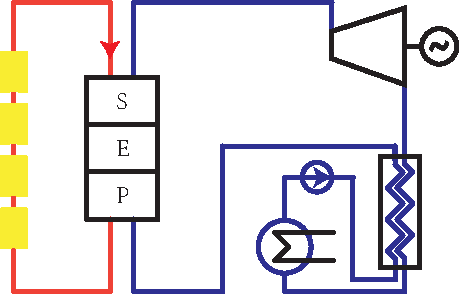
\includegraphics[width=0.7\textwidth]{fig/TypicalOrganicRankineSolarSystem}
%\caption{Schematic diagram of a typical organic Rankine cycle solar system}\label{fig:TypicalOrganicRankineSolarSystem}
%\end{figure}

Compared with steam for the Rankine cycle, it has the following advantages:
\begin{itemize}
  \item  Small turbine head allows for moderate shaft speed and a single- or two-stage design.
    \item Low volume ratio facilitates the flow path design.
    \item High volume flow and low velocity of sound results in reasonable flow areas.
    \item Low temperature drop during expansion reduces thermal stress problems.
    \item Dry expansion avoids blade erosion caused by vapor wetness.
    \item Low system pressure facilitates housing design.
  \end{itemize}

\subsection{Solar chimney}
\label{sec:sc}
Solar chimney, also known as solar updraft tower, directly (without concentration) uses the sun's heat to generate power. It uses solar radiation to increase the internal air temperature to form a flow to the chimney located at the middle of the roof. Figure~\ref{fig:SolarChimney} shows the schematic of a typical solar chimney power plant. In this plant, air is heated by the green house effect under the translucent roof. As the roof is open at its periphery, air flows into the plant due to different density distribution. Hot air flows into the chimney because of buoyancy. An electricity-generating turbine is set in the path of the air current to convert the kinetic energy of the flowing air into electricity.

\begin{figure}[!ht]
\centering 
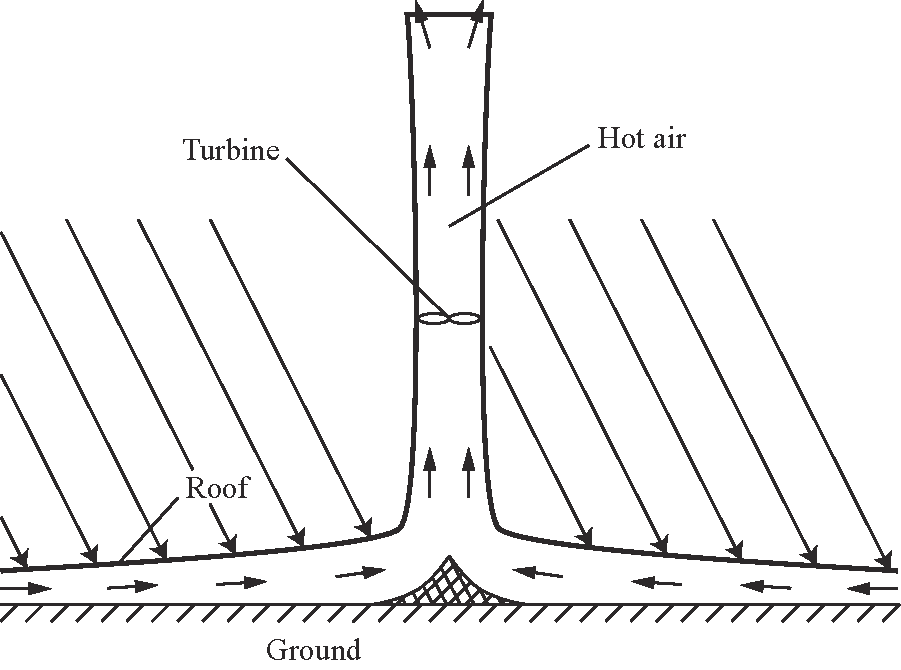
\includegraphics[width=0.7\textwidth]{fig/SolarChimney}
\caption{Schematic diagram of a solar chimney power plant}\label{fig:SolarChimney}
\end{figure}

The solar chimney can use the low temperature (low grade energy) for power generation. So the combination of parabolic trough system and solar chimney is considered an effective way for energy cascade utilization. In the combined system, the condenser in the Rankine cycle is air cooled. The fan blows the hot air that has cooled the condenser into the solar chimney power plant from its periphery. The hot air stream converges at the bottom of chimney, flows upward with the action of buoyancy and drives the turbine in the chimney.
Energy of the hot air can be utilized by the solar chimney. Figure~\ref{fig:CombinedSolarChimney} shows an example of the combined system. 

\begin{figure}[!ht]
\centering 
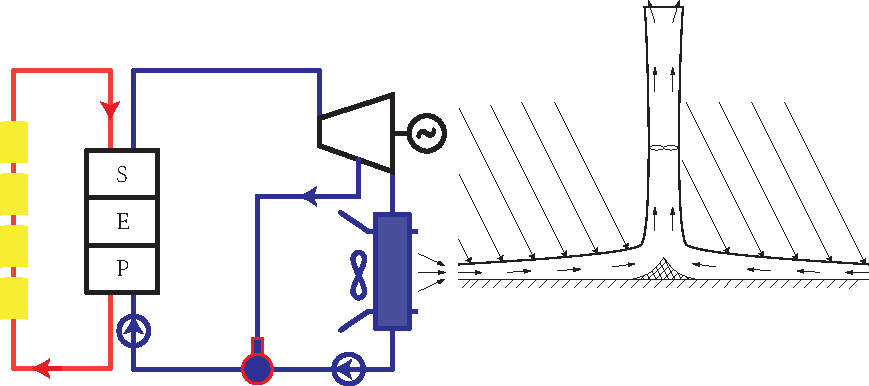
\includegraphics[width=0.7\textwidth]{fig/CombinedSolarChimney}
\caption{Schematic diagram of a combined solar trough and chimney power system}\label{fig:CombinedSolarChimney}
\end{figure}

\subsection{Collector series connection}
\label{sec:csc}
Considering different heat collecting temperatures of different types of collectors, series connection of different types of collectors can be a feasible choice for solar cascade collection. Trough collectors and Fresnel collectors have better performance for lower temperature heat collection. Dish collectors and solar towers are more suitable for higher temperature heat collection. Serial connection utilize the advantages of different types of collectors. Figure~\ref{fig:SeriesCollector} shows an example of a cascade system using collector series connection. In this system, air, the HTF, is preheated by parabolic collectors before it flows into the parabolic dish collectors.

\begin{figure}[!ht]
\centering 
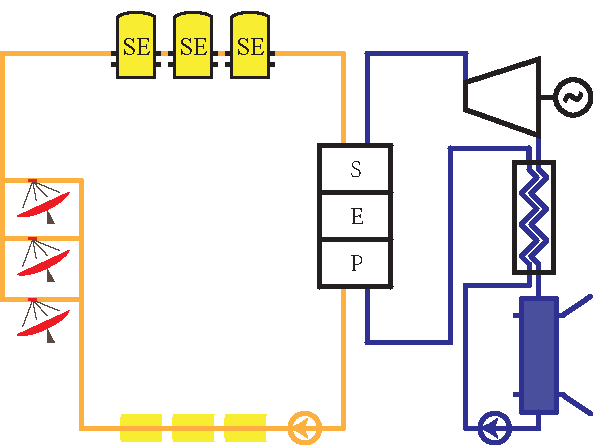
\includegraphics[width=0.7\textwidth]{fig/SeriesCollector}
\caption{Schematic diagram of a cascade system using collector series connection}\label{fig:SeriesCollector}
\end{figure}

\subsection{Direct steam generation}

All commercial parabolic trough solar plants implemented to date use heat-transfer fluid (typically synthetic oil or melton salt) in the solar field. It leads to high pressure drop, limits the oil (or salt) related equipment operation, maintenance and cost. Besides, the highest temperature of the Rankine cycle is limited by the oil (or salt) temperature. So generating steam in the receiver tubes (direct steam generation, DSG) of the solar collector is one of the directions to reduce the cost and increase the efficiency of the PTC systems. Figure~\ref{fig:DSG} shows the schematic diagram of a typical DSG solar system.

\begin{figure}[!ht]
\centering 
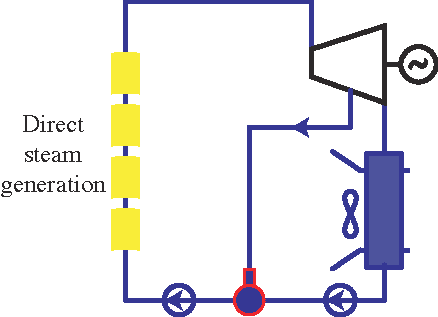
\includegraphics[width=0.7\textwidth]{fig/DSG}
\caption{schematic diagram of a typical solar system using receiver vapor generator}\label{fig:DSG}
\end{figure}

\subsection{Heat exchanger between circuits}
\label{sec:hebc}

Heat transfer between different circuits can be applied for cascade utilization of the heat collected. Depending on the two basic solar system in~\ref{fig:PTPD}, there are two types of heat exchangers that can be applied in the solar system.

In the first type, air-oil heat exchanger is applied to transfer heat between the air circuit and the oil circuit. Figure~\ref{fig:air-oil} shows an example of solar system using this type of heat exchanger. In this system, after providing heat for the Stirling engines, the hot air flows through the air-oil heat exchanger and provides heat for the oil. 

\begin{figure}[h]
\centering 
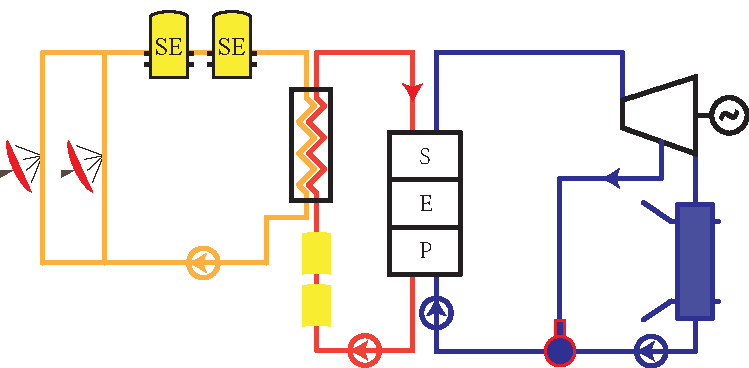
\includegraphics[width=0.7\textwidth]{fig/air-oil}
\caption{Schematic diagram of a solar system using air-oil heat exchanger}\label{fig:air-oil}
\end{figure}

In the second type, air-water heat exchanger is applied to transfer heat between the air circuit and the oil circuit. Figure~\ref{fig:air-water_1} and Figure~\ref{fig:air-water_2} show two different kinds of solar systems using this type of heat exchanger. In Figure~\ref{fig:air-water_1}, 

\noindent \begin{figure}[htbp]
\centering
	\begin{subfigure}[b]{0.4\columnwidth}
	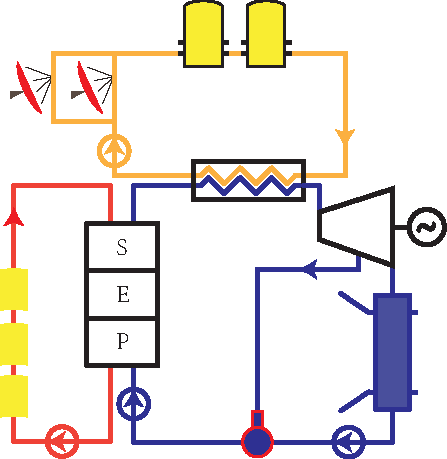
\includegraphics[width = \columnwidth]{fig/air-water1}
	\caption{}\label{fig:air-water_1}
	\end{subfigure}
	~
\begin{subfigure}[b]{0.4\columnwidth}
	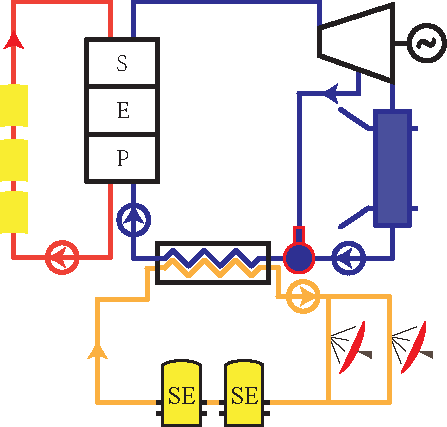
\includegraphics[width = \columnwidth]{fig/air-water2}
	\caption{}\label{fig:air-water_2}
	\end{subfigure}
	\caption{Schematic diagrams of two kinds of solar systems using air-water heat exchanger}
	\label{fig:air-water}
\end{figure}

%\begin{figure}[h]
%\centering 
%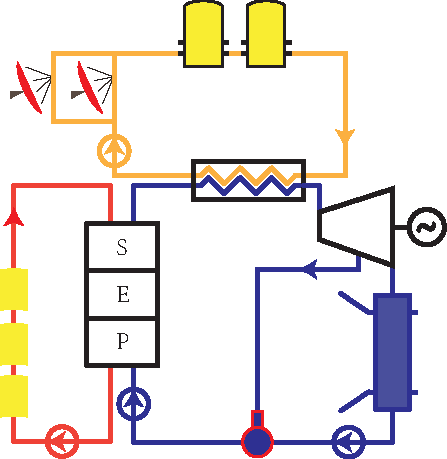
\includegraphics[width=0.6\textwidth]{fig/air-water1}
%\caption{schematic diagram of a solar system using air-water heat exchanger}\label{fig:air-water1}
%\end{figure}
%
%\begin{figure}[h]
%\centering 
%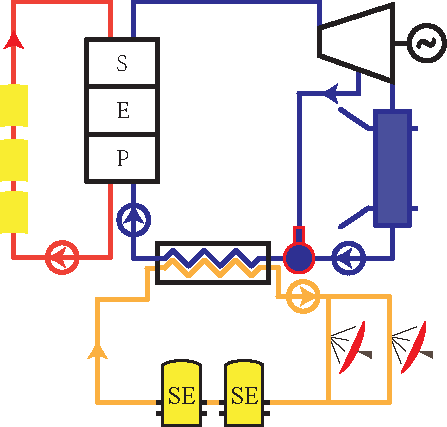
\includegraphics[width=0.6\textwidth]{fig/air-water2}
%\caption{schematic diagram of a solar system using air-water heat exchanger}\label{fig:air-water1}
%\end{figure}
\subsection{Heat recovery between cycles}
\label{sec:HRBC}

According to the second law of thermodynamics, it is impossible for any device that operates on a cycle to receive heat from a single reservoir and produce a net amount of work. For a heat engine, it requires both a hot source and a cold sink to convert heat energy to mechanical energy. 
Figure~\ref{fig:engines} shows the diagram of a typical heat engine. In a thermodynamic cycle, heat is absorbed from the hot source, only part of it can be converted into mechanical work by the engine. The ratio related to the temperatures of hot source and cold sink is fundamentally limited by Carnot's theorem.

\begin{figure}[h]
\centering 
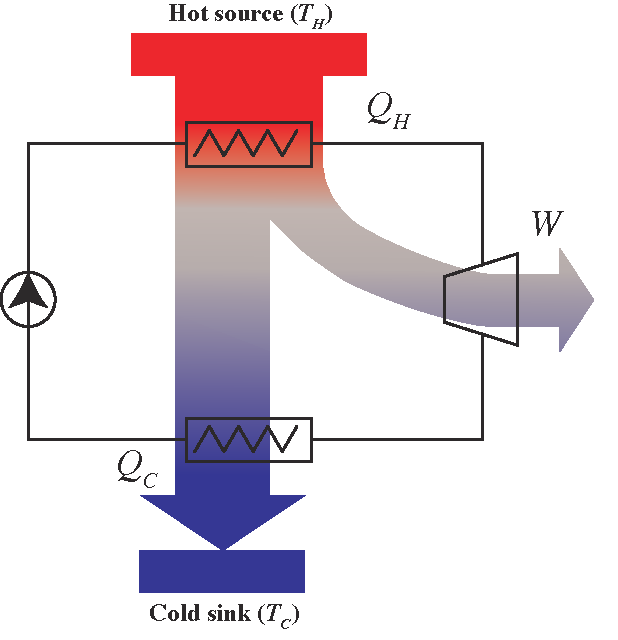
\includegraphics[width=0.7\textwidth]{fig/engines}
\caption{Diagram of a typical heat engine}\label{fig:engines}
\end{figure}

Engines that only suitable for external heating are usually considered for solar applications. Unlike an internal combustion engine that generates heat within the working fluid, an externally heated engine needs external heat to be added to the working fluid by a heat exchanger.

Three types of engines are designed to accept external heat and have been used for solar heat sources: the Rankine, the Stirling, and the Brayton cycles~\cite{Roschke1979}. The Rankine and Brayton cycles are both suitable for constant-pressure heat-addition. 
The original Brayton engine uses piston compressors and piston expanders, but more modern gas turbines and airbreathing jet engines also follow the Brayton cycle. Although the cycle is usually an open system, in order to carry out thermodynamic analysis, usually it is assumed that exhaust gases are reused as the intake so that the whole process can be analyzed as a closed cycle.
The Stirling machine uses a reciprocating piston design that allows external heating to be combined into its constant-temperature heat-addition process. 
In a Rankine cycle, the pressurized liquid enters a boiler (or a heat exchanger) where it is heated at constant pressure by an external heat source to become a dry saturated vapor.

These three kinds of cycles work at different optimum operating temperatures. Rankine cycle works with the lowest hot source temperature and Brayton works with the highest. Figure~\ref{fig:cycles} shows the diagram of the three cycles used in solar energy. The heat released by these cycles may be recovered by another cycle (bottom cycle).

\begin{figure}[h]
\centering 
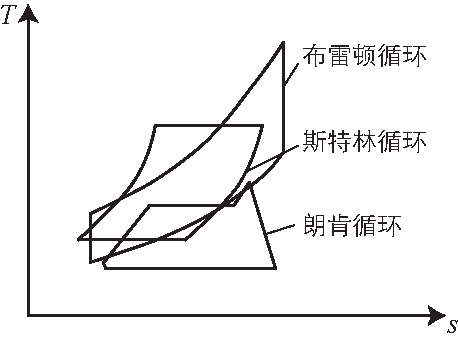
\includegraphics[width=0.7\textwidth]{fig/cycles}
\caption{Diagram of three cycles used in solar energy}\label{fig:cycles}
\end{figure}

Dunham and Lipi~\cite{Dunham2013} proposed a single Brayton and a combined Brayton-Rankine power cycle for distributed solar power generation and compared its theoretical efficiency to a single Brayton cycle. In the combined power cycle, exhaust gas of the turbine is used to provide heat for Rankine cycle. Working fluids including air, Ar, CO$_2$, He, H$_2$, and N$_2$ are examined for the topping Brayton cycle. C6-fluoroketone, cyclohexane, n-pentane, R-141b, R-245fa, and HFE-7000 are examined as working fluids in the bottoming Rankine cycle. It is found that the combination of the Brayton topping cycle using carbon dioxide and the Rankine bottoming cycle using R-245fa gives the highest combined cycle efficiency of 21.06\%, while a single Brayton cycle is found to reach a peak cycle efficiency of 15.31\% with carbon dioxide at the same design point conditions.

Bahrami et al.~\cite{Bahrami2013} proposed a combined Stirling-organic Rankine cycle (ORC) power cycle. An ORC was used as the cold-side heat rejector of a Stirling engine. The operating temperatures of the ORC are between 80$\mathrm{^\circ C}$ and 140$\mathrm{^\circ C}$ and the combined system can achieve 4\% to 8\% higher efficiency compared with a standard Stirling cycle.

Li et al.~\cite{Li2016a} proposed a novel solar electricity generation system (SEGS) using both SRC and ORC. Screw expander (SE) is employed in the SRC for its good applicability in power conversion with steam-liquid mixture. The heat released by steam condensation is used to drive the ORC. Simulation results show that efficiency of 13.68–15.62\% for the proposed system can be achieved.

Thierry et al.~\cite{Thierry2016} proposed a nonlinear optimization formulation of multistage Rankine cycle with two types of configurations. Both cascade style and series style of the ORC are considered. The results show that for some cases the multistage configurations can achieve higher efficiency at low temperature.

In our basic systems (see Figure~\ref{fig:PTPD}), Rankine cycle and Stirling cycle can be coupled for cascade usage. Figure~\ref{fig:coupledCycles} shows two configurations of the cascade systems with heat recovery between cycles.

\noindent \begin{figure}[htbp]
\centering
	\begin{subfigure}[b]{0.4\columnwidth}
	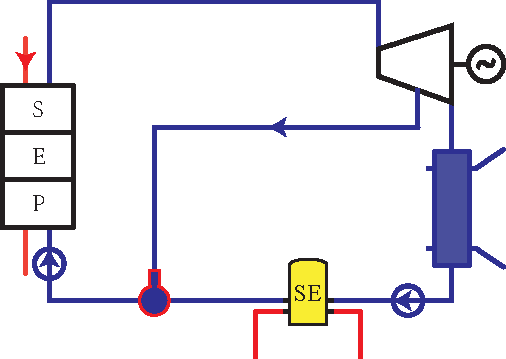
\includegraphics[width = \columnwidth]{fig/Stirling-Rankine}
	\caption{}\label{fig:air-water1}
	\end{subfigure}
	~
\begin{subfigure}[b]{0.4\columnwidth}
	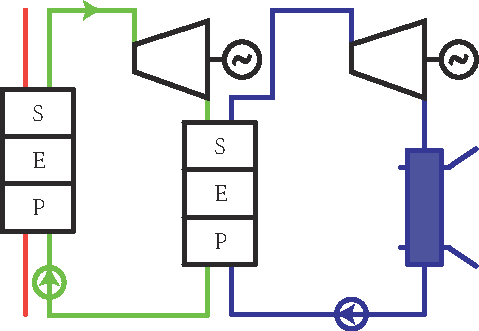
\includegraphics[width = \columnwidth]{fig/SeriesRankine}
	\caption{}\label{fig:air-water2}
	\end{subfigure}
	\caption{Schematic diagrams of two kinds of solar systems using air-water heat exchanger}
	\label{fig:coupledCycles}
\end{figure}

\section{System topology selection}
\subsection{Rankine cycle fluid}

There are two important aspects to consider when selecting the working fluid of the Rankine cycle solar power system:
\begin{enumerate}
  \item Select the working fluid that is conducive to the optimization of the cycle efficiency
  
  For a Rankine cycle solar system, the collector efficiency reduces with operating temperature, and the Rankine cycle efficiency increases with operating temperature, there exists an optimal operating temperature as illustrated in Figure~\ref{fig:Efficiency}. The working fluid should be conducive to achieve the optimal operating temperature.
  
  \begin{figure}[!ht]
\centering 
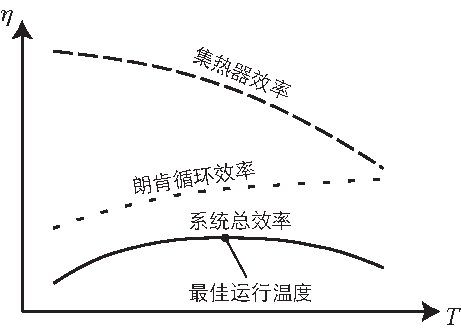
\includegraphics[width=0.7\textwidth]{fig/Efficiency}
\caption{Collector and Rankine cycle efficiency variation with operating temperature}\label{fig:Efficiency}
\end{figure}
  
  \item The working fluid state matches the heat transfer fluid state, if heat transfer fluid is used.
  
  On the one hand, the operating temperature of the working fluid should be lower than the collecting temperature of the HTF. On the other hand, the operating temperature of the working fluid should not be much lower than the collecting temperature of the HTF to avoid large exerge loss during the heat exchange process.
  
\end{enumerate}

Based on the advantages and disadvantages of water and organic fluid as the working fluid of Rankine cycle, it is clear that, for low operating temperature and small capacity distribution power generation, organic fluid will be a better choice, otherwise water is the better one. Bao and Zhao~\cite{Bao2013} presented a comprehensive review of working fluid selection (including pure fluids and mixtures). In this review, many factors such as operating conditions, working fluid characteristics, equipment structures and environmental safety considerations were considered.
It has to be mentioned that the types of working fluids (mainly dry or wet) will affect the operation and layout of the system.

\subsection{Solar chimney}

Section~\ref{sec:sc} shows the idea of coupling solar chimney to concentrated solar thermal power generation technologies.
However, the efficiency of current solar chimney system is still very low. Primary design data of solar chimney power plants with different location, different chimney height and collector height are shown in Table~\ref{tab:sc}~\cite{Bilgen2005}. The preliminary design parameters in Table~\ref{tab:sc} are selected and determined for a nominal solar intensity of 1000$\,\mathrm{W/m^2}$ and the nominal plant power of 5$\,\mathrm{MW}$. From the table, it can be found that the chimney efficiency and total efficiency are very low and the technology is still in the development stage.
\begin{table}[htbp]
	\caption{Results of SEA models under specified parameters}
	\begin{center}
	\begin{tabular}{ccccc}
		\toprule
		&Ottawa    &Winnipeg    &Edmonton    &Schlaich\\
		\midrule
		Collector diameter (m)    &-&-&-&1110 \\
  Collector area ($\mathrm{m^2}$)    & 950000    & 950000&950000&950000\\
  Chimney height (m)    &123    &60    &    35&    547\\
  Collector height (m)    &848    &975    &1024    &    -\\
  Chimney diameter (m)    &54    &54    &54    &54\\
  Temperature rise in collector ($\mathrm{^\circ C}$)    &25.9    &25.9    &25.9    &25.9\\
  Updraft velocity (m/s)&9.1    &9.1    &9.1    &9.1\\
  Total pressure head (Pa)&518.3    &518.3    &518.3    &383.3\\
  Average efficiency\\
  Collector (\%)    &56.00    &56.00    &56.00    &56.24\\
  Chimney (\%)    &1.82    &1.82    &1.82    &1.45\\
  Turbine (\%)    &77.0    &77.0    &77.0    &77.0\\
  Whole system (\%)    &0.79    &0.79    &0.79    &0.63\\
		\bottomrule
	\end{tabular}
	\end{center}
	\label{tab:sc}
\end{table}

%Besides, it will cost much more to apply a chimney tower in the demonstration system of this project. 
Besides, a solar chimney is costly and requires vast land, which is adverse to the future deployment of solar cascade demo system. With these considerations, the solar chimney plans are not adopted. 

\subsection{Collector series connection}
Each type of collector has its own suitable temperature range. It is feasible to heat the HTF step by step using different types of collectors with series connection.

It can be a good choice to apply flat plate solar collectors and parabolic trough collectors in traditional solar tower power plant that uses water as the HTF (such as Solar One). As demonstrated in Figure~\ref{fig:seriesCollection}, condensed water is heated by the flat plate solar collectors and feedwater is heated by the parabolic trough collectors. Flat plate collectors and parabolic trough collectors have much lower unit thermal cost compared to solar tower. The addition of flat plate collectors and parabolic trough collectors can effectively reduce the cost of the system.

\begin{figure}[!ht]
\centering 
\includegraphics[width=0.7\textwidth]{fig/SeriesCollection}
\caption{Schematic diagram of a cascade system using collector series connection}\label{fig:seriesCollection}
\end{figure}

A collector series connection is proposed in Section~\ref{sec:csc} (see Figure~\ref{fig:SeriesCollector}) depending on the basic systems. In this configuration, air is heated in the trough collectors and dish receivers consequently. After providing heat for the Stirling engines, the hot air flows into the heat exchanger to provide heat for the Rankine cycle. However, this topology is not adopted due to the parabolic trough collectors. In this collectors, air is used as the HTF, which will lead to low efficiency due to low conductivity and low heat capacity.

\subsection{Direct steam generation}
Direct steam generation for solar thermal power generation has the advantage of having fewer components and no loss of temperature required with an intermediate transfer.  Besides, it is clear that water is characterized by lower environmental risk than thermal oil so that leakages in a DSG power plant do not represent an environmental hazard ~\cite{Fernandez2010}. Water has a lower freezing temperature than thermal oil and above all than solar salt: the efforts required to ensure adequate anti-freezing protection are significantly reduced. Water is also less corrosive than solar salt~\cite{Giglio2017}. With both liquid and vapor in a receiver, however, extreme care must be taken in the design of the receiver to ensure that the radiant flux incident on that portion of the receiver containing vapor is less than the flux incident in the regions with liquid and where boiling is taking place. This is because the heat-transfer coefficient into a liquid is significantly higher than into superheated vapor. For similar values of solar flux, burnout of the receiver walls could occur in the regions where vapor exists on the other side of the receiver wall.

Many concentrating collector designs require that the receiver change attitude while the collector tracks the sun. This change of attitude increases the chances of high flux on portions of the receiver containing vapor.
Two examples of solar Rankine power systems where the engine working fluid vapor is generated directly in the receiver are the Solar One Pilot Plant at Barstow, CA and the solar organic Rankine cycle module built by Ford Aerospace and Communications Corporation. Because Solar One is a central receiver system, the vertical-tube receiver remains stationary and liquid level control is relatively easy. The vertical tubes of the receiver are made of a material with a high melting point and thus can withstand high temperatures in the upper regions where vapor is being superheated. Tube burnout is avoided in the Ford Aerospace receiver design because the inner wall of the receiver is a copper shell with tubes wound around its exterior. The high thermal conductivity of the copper shell provides an averaging effect on receiver temperature, and superheat is attained without burnout of the receiver walls.

All the CSP commercial plants already built apply indirect steam generation, with the exception of the 5 MWe DSG Thai Solar One (TSE-1) plant in Thailand (Thailand, 2012)~\cite{Khenissi2015}. The reason for this universally accepted choice must be found in the difficulties related to the flow control and manufacturing of equipment to be used in the presence of a two-phase flow in the absorber tubes. The behavior of the two-phase flow inside the absorber tubes of a parabolic-trough collector forces the implementation of a complex and expensive control system and the use of fast water streams in order to avoid stratified flow.
			
Another problem related to the DSG is the high value of the steam pressure inside the receiver tubes that must match the turbine inlet pressure for less than pressure losses. Indeed, handling the moveable and flexible components forming the receiver tube of the collector in case of high-pressure values was one of the main problems to be faced at the early stages of the DSG concept technology. 

Apply direct steam generation may be a better choice in the cascade system, however, it is not adopted for the cascade system for its immaturity.

\subsection{Heat exchanger between circuits}

Section~\ref{sec:hebc} introduces two types of heat exchangers that may be applied in the solar thermal cascade system -- the air-oil heat exchanger (see in Figure~\ref{fig:air-oil_c}) and the air-water heat exchanger (see in Figure~\ref{fig:air-water_c}). 

\begin{figure}[h]
\centering 
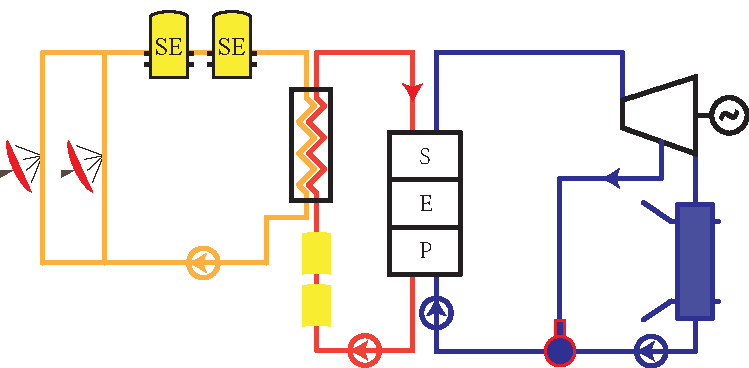
\includegraphics[width=0.7\textwidth]{fig/air-oil}
\caption{Schematic diagram of a solar system using air-oil heat exchanger}\label{fig:air-oil_c}
\end{figure}

\noindent \begin{figure}[htbp]
\centering
	\begin{subfigure}[b]{0.4\columnwidth}
	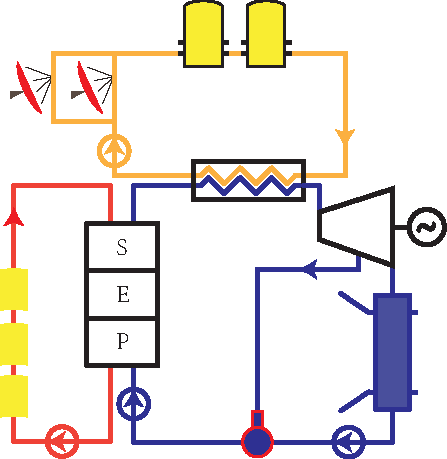
\includegraphics[width = \columnwidth]{fig/air-water1}
	\caption{}\label{fig:air-water_1_c}
	\end{subfigure}
	~
\begin{subfigure}[b]{0.4\columnwidth}
	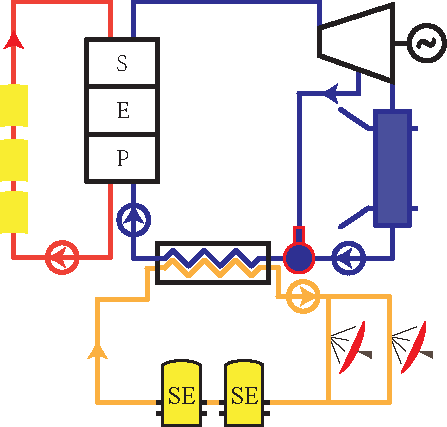
\includegraphics[width = \columnwidth]{fig/air-water2}
	\caption{}\label{fig:air-water_2_c}
	\end{subfigure}
	\caption{Schematic diagrams of two kinds of solar systems using air-water heat exchanger}
	\label{fig:air-water_c}
\end{figure}

For the first type, air provides heat for oil. It is not economic for several reasons. First, The temperature of the heat transfer oil can not be further increased. The temperature of the oil is not limited by the parabolic trough collectors. The temperature of the oil is constrained by the oil properties and heat collecting temperature of the trough collectors can exceed this value. In high temperature conditions, oil may deterioration, evaporation, decompose, which has a negative impact on the stable and safe operation of the system. Second, using dish to provide heat for the oil is not suitable since the dish is designed for higher temperature collections and it's less cost-effective compared with parabolic trough.

For the second type, air provides heat for water. Two kinds of solar systems using air-water heat exchanger can be found in Figure~\ref{fig:air-water_c}. Figure~\ref{fig:air-water_1_c} shows the scheme that air after the Stirling engine is used to overheat the steam. It's feasible since the air can increase the average temperature of the endothermic process of the water to increase the efficiency of Rankine cycle. On the other hand, in the traditional solar trough system, the main steam temperature is limited by the oil, which is not conductive to Rankine cycle efficiency. In this proposed cascade system, the main steam temperature of the Rankine cycle can be raised to be higher than 400$\mathrm{^\circ C}$ to eliminate the negative effect of the oil.
This is the scheme that will be discussed in detail in the next few chapters. Figure~\ref{fig:air-water_2_c} shows the scheme that air after the Stirling engine is used to preheat the feed water. It is not a good choice since the temperature difference of the heat transfer process is large and it provides no benefits to increase the inlet temperature of the steam turbine.
 
\subsection{Heat recovery between cycles}
As it is mentioned in section~\ref{sec:HRBC}, 
\section{Selected system topology}